%% ****** Start of file aiptemplate.tex ****** %
%%
%%   This file is part of the files in the distribution of AIP substyles for REVTeX4.
%%   Version 4.1 of 9 October 2009.
%%
%
% This is a template for producing documents for use with 
% the REVTEX 4.1 document class and the AIP substyles.
% 
% Copy this file to another name and then work on that file.
% That way, you always have this original template file to use.

%\documentclass[aip,graphicx]{revtex4-1}
%\documentclass[aip,reprint]{revtex4-1}

%\usepackage{graphicx}

%\draft % marks overfull lines with a black rule on the right
%\documentclass[pre,aps,floatfix,authordate1-4,twocolumn]{revtex4-1}
%\documentclass[pre,aps,floatfix,authordate1-4]{revtex4-1}

\documentclass[aip,jcp,twocolumn]{revtex4}
%\documentclass[aip,jcp]{revtex4}
%\documentclass{article}



%\documentclass[aps,prl,preprint,groupedaddress]{revtex4}

\usepackage{rotating} 
\usepackage{times}
\usepackage{graphicx}
\usepackage{setspace}
\usepackage{amsmath}
\usepackage{epstopdf}
\usepackage[obeyFinal]{easy-todo}
\usepackage{csquotes}
\usepackage{mhchem}

%\usepackage{markdown} 

\begin{document}

% Use the \preprint command to place your local institutional report number 
% on the title page in preprint mode.
% Multiple \preprint commands are allowed.
%\preprint{}

\title{Accurate binding of calcium to phospholipid bilayers by effective inclusion of electronic polarization} %Title of paper

% repeat the \author .. \affiliation  etc. as needed
% \email, \thanks, \homepage, \altaffiliation all apply to the current author.
% Explanatory text should go in the []'s, 
% actual e-mail address or url should go in the {}'s for \email and \homepage.
% Please use the appropriate macro for the type of information

% \affiliation command applies to all authors since the last \affiliation command. 
% The \affiliation command should follow the other information.

\author{Josef Melcr}
\author{Hector Martinez-Seara Monne}
\author{Pavel Jungwirth}
\affiliation{Institute of Organic Chemistry and Biochemistry,
Academy of Sciences of the Czech Republic, 
Prague 6, Czech Republic}

\author{O. H. Samuli Ollila}
\email[]{samuli.ollila@helsinki.fi}
%\homepage[]{Your web page}
\affiliation{Institute of Organic Chemistry and Biochemistry,
Academy of Sciences of the Czech Republic, 
Prague 6, Czech Republic}
\affiliation{Institute of Biotechnology, University of Helsinki}


% Collaboration name, if desired (requires use of superscriptaddress option in \documentclass). 
% \noaffiliation is required (may also be used with the \author command).
%\collaboration{}
%\noaffiliation

\date{\today}

\begin{abstract}
% insert abstract here
Classical molecular dynamics simulations give detailed information about membrane structure and dynamics. 
However, there is still a room for improvements in current force fields – it is known from the literature, that the binding of ions, especially cations, to phopholipid membranes is overestimated in all classical models [1]. 
We suggest that the membrane-ion interactions can be corrected by including implicit electronic polarizability into the lipid models through the electronic continuum correction (ECC) [2], which was already applied to monovalent and divalent ions yielding models that feature correct ion pairing [3]. 
Using the electrometer concept [3, 4] and x-ray scattering form factors, our simulations point out that our hypothesis is correct and ECC is indeed a missing important contribution in current classical lipid models. 
Moreover, the solid physical principles behind ECC are found not to hamper other relevant properties of a phospholipid bilayer. 
The new lipid model, "ECC-lipids", shows accurate binding affinity to sodium and calcium cations and headgroup order parameter response to bound charge. 
We also provide for the first time a realistic stochiometry of bound calcium cations to a POPC membrane, and their binding sites. 
This work will continue as an open collaboration project NMRlipids IV (http://nmrlipids.blogspot.fi).

[1] Catte, A., Girych, M., Javanainen, M., Melcr J., Miettinen, M. S., Oganesyan, V. S. and Ollila H. S.,  PCCP 18(47) 32560-32569 (2016)
[2] Leontyev, I. V., and Stuchebrukhov, A. A., JCTC 6(5) 1498–1508 (2010)
[3] Kohagen, M., Mason, P. E., and Jungwirth, P., J. Phys. Chem. B 120(8) 1454–60 (2015)
[4] Seelig, J., MacDonald, P. M., and Scherer, P. G., Biochemistry 26(24) 7535–7541 (1987)
\end{abstract}

%\pacs{}% insert suggested PACS numbers in braces on next line

\maketitle %\maketitle must follow title, authors, abstract and \pacs

% Body of paper goes here. Use proper sectioning commands. 
% References should be done using the \cite, \ref, and \label commands


% Here I write pseudo-article statements that will make the main argument.
% Beautiful polished sentences will be formed only afte we agree on these basic things
\section{Introduction}

 motivation, significance of membranes, phospholipids and simulation.

 assumptions (so that we have structure of the paper like in a mathematical proof) -- 
 MD simulation is a good tool for studying molecules.
 classical MD models can describe lipids accurately, 

 MD is ... and it serves ... it is useful for ... (describe throuhg references)

 Lipid membranes, especially phospholipid membranes; their significance for life, sciences, society, pharma ...

%\textbf{Specific introduction: current FFs and MDEC/ECC}

 Current force fields -- pros and cons, at a good shape in many aspects, agree on various properties.  -- write basic ideas from the lipid-FF whitepaper I did recently.

 lipid force fields fail in description of membrane-cation interaction -- could be answered by ECC? 
Cations were shown to generally overbind in PC lipid bilayers in NMRlipids II project. 
Here we propose that the cation overbinding can be corrected by implicitly inducing electronic polarizability in lipid headgroups by scaling the partial charges -- i.e. MDEC/ECC~\cite{leontyev11}\todo{Bulid BibTex references database.} paradigm.

MDEC -- or -- ECC 
\todo{choose one}{We have to decide whether we will refer to the method as a correction (ECC) or as a MD simulation paradigm (MDEC) -- and choose on of these labels. -- Joe: use ECC as we apply MDEC rather as a correction to current state not as a new paradigm for FF development.}
MD in electronic continuum as in \cite{leontyev11} or electronic continuum correction as in \cite{Jungwirth2015}

Describe ECC: good physical concept for treating part of the polarizability (electronic) in a simple mean-field way.

Succesful application: Works for cations \cite{Jungwirth2015,kohagen14,kohagen16}\todoii{REF}{Missing references} -- motivation for its application to zwitterionic lipids like POPC.

Hypothesis: ECC helps in describing even zwitterionic molecules like POPC, will be demonstrated through headgroup order parameter response to cationic molecules.

\section{Methods}

Simulations with molecular mechanics models represent nuclei as classical particles 
and describe their interactions through a pariwise additive empirical potential \cite{SOME_review, FF_papers}. 
According to the electronic continuum correction (ECC), electrons that surround 
the nuclei shall be taken into account in such simulations as an electronic continuum. \cite{leontyev11}
Such a continuum responds to the electrostatic interactions of the explicitly represented nuclei
as a polarizable dielectric. 
The dielectric constant of shuch a dielectric medium, $\epsilon _{el}$, will 
then resduce the electrostatic interactions in between the nuclei. 
This can be formally represented in classical simulations through scaling of charges of particles with a factor $f_q = \epsilon _{el} ^{-1/2}$. 
Note that the high frequency dielectric constant, which is experimentally measurable \cite{some_original_work, leontyev11}, represents
the part of dielectric response only due to electrons, and it is approximately $\epsilon _{el} ~ 2$ for almost any biomaterial that is
usually simulated/exists in a living cells \todo{choose between the two options}.
The high frequency dielectric constant of water, 
the most abundant molecule in any simulaiton in biophysics, 
is $\epsilon _{el} = 1.78$, hence the scaling factor adopts the value of $f_q = 0.75$. \cite{some_orig_source, leontyev11}

The newly presented ECC-POPC model is based on the POPC model from Lipid14~\cite{dickson14} force field. 
There, the partial atomic charges were derived by 
fitting the electrostatic potential of its model quantum chemistry representation in vacuum. 
If such charges are obtained in an implicit solvent, they vary the most for the polar moieties \cite{maiejewski14}. 
In order to represent this difference in polarity in a model with fixed charges, 
we shall use the average charges from both environments (IpolQ charges) \cite{Cerutti2013}. 
By taking the charges of oxygen atoms in vacuum and implicit water solvent for POPC from \cite{maciejewski14}, 
we represent the IpolQ charges in the electronic continuum correction of the Lipid14 model
by increasing the scaling factor for charges to $f_q = 0.8$. 

Because the biologically relevant cations like \ce{Na^+} and \ce{Ca^{2+}
are found to interact only with the phospholipid head group,
and the accuracy of alkyl sidechains in Lipid14 model are satisfactory, 
we exclude alkyl tails from our modifications. 

By scaling the particle charges alone, we reduce the 
electrostatic interactions and, hence, their contribution to hydration.
A simple approach to correct for this effect is to scale also 
the sigma factors in the Van der Waals interaction that is 
modelled with a Lennard-Jones potential. \cite{lennard-jones_work}
In line with the electronic continnum correction,
the scaling factor for sigma parameters, $f_\sigma$,
has to lay between $f_q$ and 1.

The optimal value for $f_q$ was found by matching the overall membrane structure, 
scattering form factors to the experimental data.
This ensures that the presented model describes the membrane strucutre correctly,
adopts correct liquid disordered phase, 
and provides area per lipid agreeing with experiments (see Fig~\ref{simVSexpNOions} and Table~\ref{tab:apls}). 


Detailed and robust structural information of lipid bilayers can
be reached with C-H bond order parameter from NMR experiments,
which tell on the lipid structure sampled by each individual molecule.
On the other hand, form factors from scattering experiments validate overall bilayer properties, 
lateral density (area per molecule) and thickness \cite{ollila16}. 
The structural quality of
new ECC lipid model is evaluated against scattering form factors and NMR order parameters
in Fig. \ref{simVSexpNOions}
\todo{Add acyl chain order parameters, POPC chemical structure}
\todo{Why original Lipid14 model seems to deviate from experiments, in contrast to the original publication? Different simulation setup used?}
\begin{figure}[]
  \centering
  \includegraphics[height=8.5cm,angle=-90]{../Fig/form-f_exp-l14-eccl17.eps}
%  \caption{\label{fig:form-f}
%    X-ray scattering form factors from experiments~\cite{Kucerka2011} and simulations using Lipid14 and ECCLipids17 models.  }
%\end{figure}
%
%\begin{figure}[]
%  \centering
  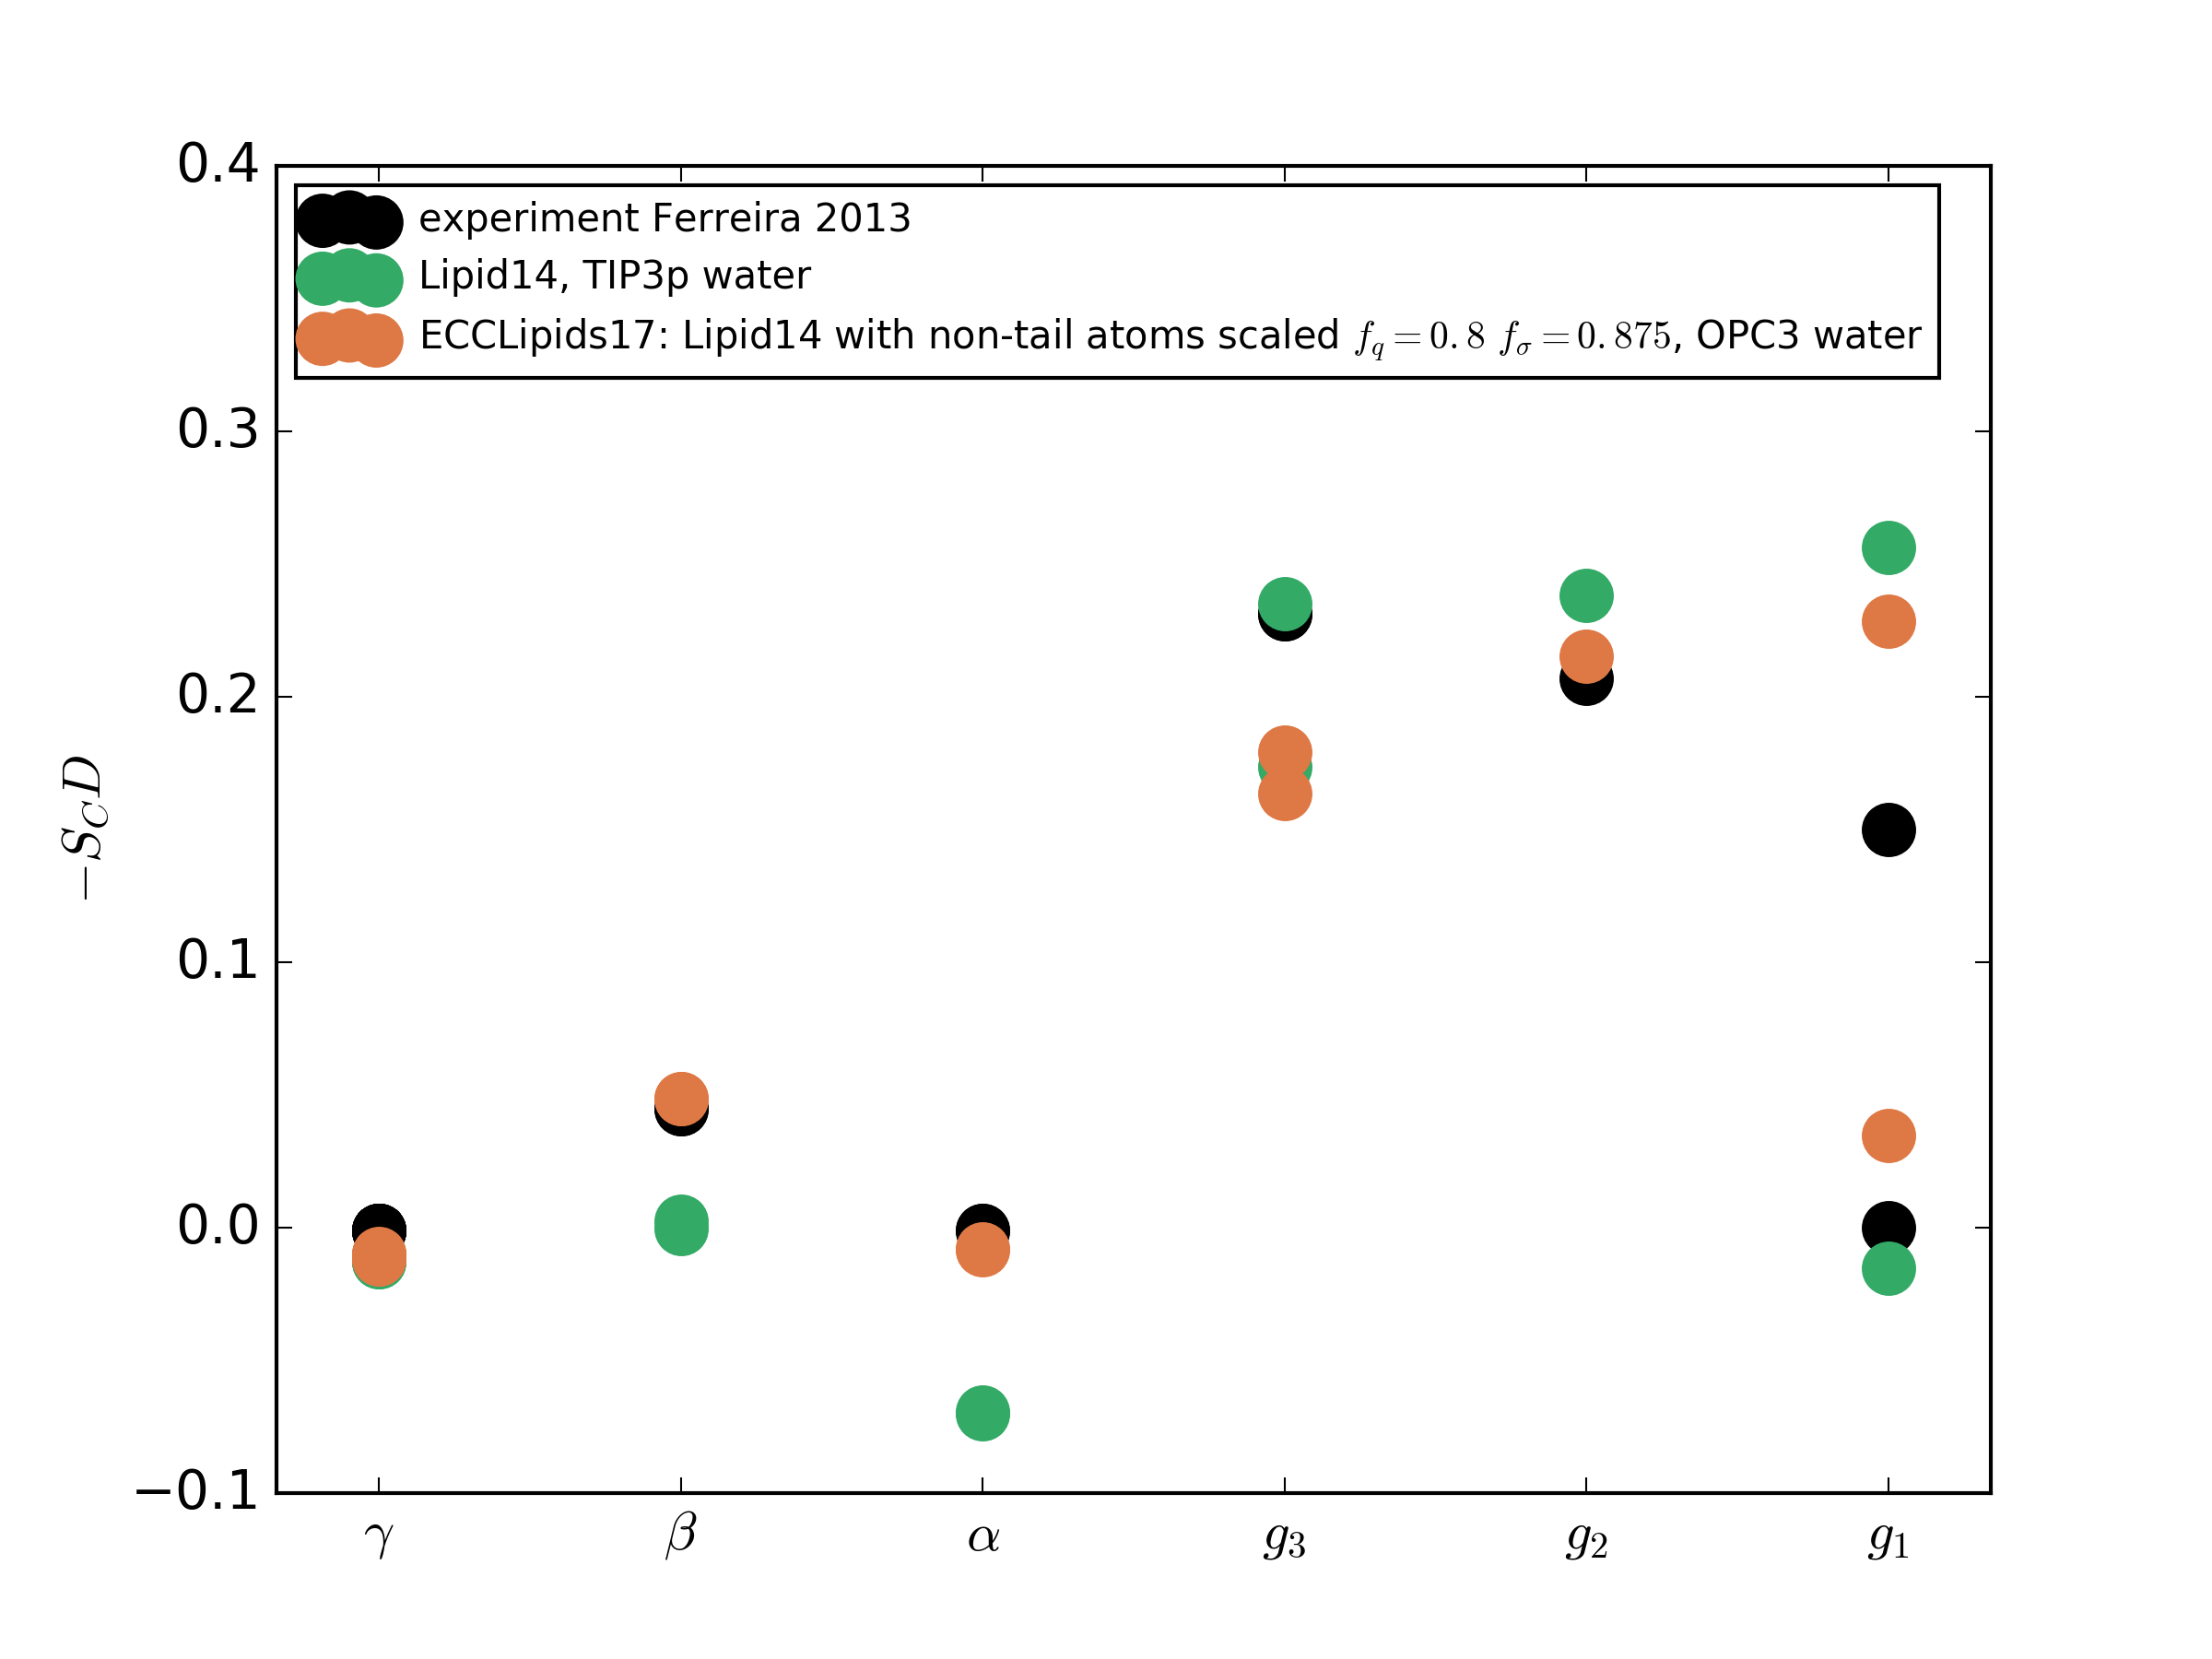
\includegraphics[width=9.0cm]{../Fig/ipython_nb/Headgr_OPs_exp-L14-ECCL17.png}
  \caption{\label{simVSexpNOions}
    X-ray scattering form factors from experiments~\cite{Kucerka2011} and simulations using Lipid14 and ECCLipids17 models. 
    Headgroup and glycerol backbone order parameters from simulations with Lipid14 \cite{dickson14} and EECLipid17 models
    compared with experimental order parameters from \cite{ferreira13}.}
\end{figure}
Area per molecules extracted from MD simulations and SPD model fitted to scattering data \todo{check that this the case for the used values}
are shown in Table \ref{tab:apls}.
\todo{finalize figure (NMR headgr. OPs + SAXS, continue in the discussion.}
\begin{table}
  \caption{Area per lipid from different models for POPC without ions\label{tab:apls} }
  \begin{tabular}{c c c}
    model          & A (Å$^2$)   & Temperature [K] \\
    \hline
    Lipid14 (literature)  & 65.6$\pm$ 0.5  &  303 \\
    Lipid14ecc0.80+sigma0.875 &        &  313    \\
    GMX small patch           & 64.9   &         \\
    GMX 4xbig patch           & 65.5   &         \\
    oMM small patch           & 63.65  &         \\
    oMM 4xbig patch           & 63.7   &         \\
    \hline
    experiment \cite{Jambeck2012}\todoii{REF}{put original references, not Slipids param. paper.}  & 62.7  &  293    \\
    experiment  & 64.3  &  303    \\
    experiment  & 67.3  &  323    \\
    experiment  & 68.1  &  333    \\
    experiment POPE  & 56.6 &  303    \\
    \hline
  \end{tabular}
\end{table}



Ion binding in lipid bilayers can be accurately measured and compared
between experiments and simulations by using lipid headgroup order
parameters and ''electrometer concept'' introduced by Seelig et al. \cite{seelig87,catte16}.
This is based on the experimental observations that order parameters
for $\alpha$ and $\beta$ carbons are proportional to the amount of bound charge
in lipid bilayer, which was rationalized as a charge induced tilt
of the headgroup dipole \cite{seelig87}. Later analysis including signs of the order
parameters showed that the order parameters are actually decreasing with bound
positive charge and {\it vice versa} for negative charge \cite{ollila16,catte16}.
To date, there is no lipid model that can describe such a behaviour, 
the electrometer response and cation binding, quantitatively well~\cite{catte16}

\section{Results and Discussion}

Order parameter changes from experiments \cite{seelig87} and simulations with Lipid14 model and with ECC-lipids model 
as a function of bound charge are shown in Fig. \ref{OrderParameterCHANGESnewMODELS}. 
Approximately linear decrease of headgroup order parameters is observed both 
in simulations and experiments with the cationic surfactant (dihexadecyldimethylammonium bromide, C$_{12}$Cl$_{16}$$^+$N2C$_1$Br$^-$). 
The use of a cationic surfactant has the benefit that it is not a subject of partitioning between water and lipid phase. 
This means that we know the exact amount of bound charge in the membrane both in experiment and simulation. 
Quantitative comparison reveals that in the original Lipid14 model the response is overestimated for both order parameters, $\alpha$ and $\beta$. 
This suggests that the observed overestimated response in \cite{catte16} 
is at least in part due to the high sensitivity of the headgroup order parameter response, 
not only due to overestimated binding of cations. 
Secondly, the $S^\alpha/S^\beta$ ratio of the response is found to be slightly larger than in experiments (VALexp vs VALsim\todoi{Add values of $S^\alpha/S^\beta$ response for sim and experiment}).
This property is kept also by the newly derived model, ECC-lipid, and, hence, 
it shows a perfect agreement in the response of the headgroup order parameter $S^\alpha$ 
but underestimates slightly the response of $S^\beta$. 


\todo{ongoing,Actual concentration of cations in simulation has yet to be estimated. 
If it varies too much from the nominal concentration, I may need to tweak the scaling factors, $f_q$ or only $f_\sigma$, to accomodate it. 
However, it is very unlikely, response to the surfactant \ce{DHMDMAB} is OK. 
Big patches with loads of solvent are running at the moment to guide me on the possible finite-size errors and this conc-error.} 

\begin{figure*}[]
  \centering
  \includegraphics[width=16.0cm]{../Fig/OrdParChanges_NaCl_CaCl2_surf.eps}
  \caption{\label{OrderParameterCHANGESnewMODELS}
    Headgroup order parameter changes as a function of NaCl, CaCl$_2$ concentration and
    cationic surfactant (dihexadecyldimethylammonium bromide, C$_{12}$Cl$_{16}$$^+$N2C$_1$Br$^-$)
    from simulations and experiments (DPPC \cite{akutsu81}, POPC \cite{altenbach84}, surfactant \cite{scherer89}).
    Simulations with Lipid14 and Åqvist ion model from \cite{catte16,lipid14POPC0mMNaClfiles,lipid14POPC350mMCaClfiles,lipid14POPC1000mMCaClfiles}.
  }
  \todoii{Add Lipid14-Aquist data.}{Lipid14/Åqvist data to be added from https://github.com/NMRLipids/lipid\_ionINTERACTION/blob/master/Data/POPC/CaCl/LIPID14/LIPID14caclCONSchange.dat . Joe: I'm not sure what is meant -- I think Aquist data are actually plotted there. I recently changed it to L14+Dang ions (both data and plot). I think just one ion model is sufficient (and ECC-ions are based on Dang model).}
\end{figure*}

Ion density profiles between different simulation models are compared in Fig. \ref{fig:cacl-dens}.
Density profiles from simulations with original Lipid14 and Dang ions \cite{smith94,chang1999,dang2006} 
show a pronounced peak in the position of the phosphate moieties of POPC. 
The use of a ECC-ion model~\cite{kohagen14,kohagen16} along with original Lipid14 does not significantly change it. 
The new ECC-lipid model with scaled ions exhibits on the other hand smaller density in this region 
suggesting overall weaker binding of cations (Fig.~\ref{OrderParameterCHANGESnewMODELS}). 
This demonstrates how importnat it is to account for electronic polarizability also in molecules with zero total charge. 
Alltogether,
the response of headgroup order parameters as a function of CaCl$_2$ concentration is in agreement with
experiments in the new ECC-lipid model simulated with ECC model of CaCl$_2$. 
This is a significant improvement
over previous models available for lipid--ion interactions studies \cite{catte16} and indicates that
the new model can be used for detailed studies of lipid-ion interactions.

\begin{figure}[]
  \centering
  \includegraphics[width=9.0cm,angle=0]{../Fig/CAdensities.eps}
  \caption{\label{fig:cacl-dens}
    Density profiles of \ce{Ca^{2+}} and \ce{Cl^-} for Lipid14 model with Aquist parameters and with ECC ions and ECCLipids17 with ECC ions. }
\end{figure}


One possible example is to adress the discourse on the stoichiometry of \ce{Ca^{2+}} binding to POPC~\cite{Altenbach84} \todoii{REFs}{Add references on Ca2+:POPC stoichiometry}. 
In line with the early experimental finding~\cite{Altenbach84}, we find that our data 
fit well a ternary complex model, which assumes 2 POPC molecules per 1 \ce{Ca^{2+}}. 
In contrast to this experiment, however, we possess also a complete atomistic detail of this phenomenon.
Hence we can support this empirical finding with a direct observation of transient complexes of \ce{Ca^{2+}} and POPC.
The simulation suggests that the stoichiometry 2~POPC:1~\ce{Ca^{2+}} is the most common complex. 
In addition, there also is a non-negligable probability of one \ce{Ca^{2+}} cross-bridging three POPC molecules. 
This cannot be observed in experiments without atomistic detail as it makes only a small perturabation to the binding isotherm that assumes 2~POPC per 1~\ce{Ca^{2+}}. 
\todo{Analyze stoichiometry for \ce{Na^+}, \ce{Ca^{2+}}, their interaction energies with the lipid membrane, etc, and finalize the discussion after these results.}

It is also suggested that the addition of \ce{NaCl} to the solution of \ce{CaCl_2} enhances the hedgroup order parameter response compared to the solution with only \ce{CaCl_2}. \cite{Altenbach84}
\todo{Simulate this effect and discuss it further}

\todo{The difference between DPPC and POPC -- simulate and compare with experiment. }

\begin{figure}[]
  \centering
  \includegraphics[height=9.0cm,angle=-90]{../Fig/bound-CAs_conc-eccl17.eps}
  \caption{\label{fig:cacl-bind}
    Binding isotherm assuming stoichiometry of 2~POPC:1~\ce{Ca^{2+}} as used in \cite{Altenbach84} fits the simulation data nicely.}
\end{figure}



\textbf{Discussion:}

\todo{It might be worth acknowledging each experimental finding in \cite{Altenbach84} and observations in \cite{Javanainen2017-ChemComm}.}

other lipids: charged lipids? -- ongoing research in our lab.
I'm currently working on POPE with Aniket for curved (and flat) membranes. 

Samuli: From the point of view of this paper, the most relevant other lipid to study would be DPPC to see if we can reproduce the difference between POPC and DPPC in experiments.

Joe: In addition, there are more experimental OP data on DPPC. However, it is not necessary and we can leave it to the community project. 

Role of water model: we use OPC3 (current best), it would be worth giving an estimate how results change when we use say SPCE or even TIP3p at least in the SI (so that the reader knows what errors to expect comming from these sub-optimal models). 
In addition, there is protein force field Amber15-FB, which uses water close to OPC3, TIP3pFB \todoii{REFs}{add references here}.
On the other hand, it might be the best if we used a model that doesn't have the dielectric constant from nuclei 78, but rather 44 -- TIP4p2005 is the closest. \cite{OPC_paper, ForceBalance_paper}

questionable charge distribution from RESP -- a leeway for further tweaks of the FF.
It is not obvious that RESP charges provide the best description, especially due to its non-uniqe solution. 
Shall we solve RESP fitting with the constraint of full charges and then scale down, or shall we rather solve the fitting with a scaled total charge target?

acheivable accuracy of the MD engines themselves (mainly Hector's worry) is another limiting factor in fine tuning parameters -- solid physical ground helps.

application of the correction to other lipid models: The rule looks general, however, it depends on how accurate the original model was.
From preliminary simulations with POPE, it looks that the rule works for Lipid14 FF, at least for zwitterionic headgroups.

\section{Conclusion}

%Reiterate what we did...
We present models of POPC and DPPC lipids that for the first time exhibit accurate headgroup order parameter response to cation binding. 
The models are derived from Lipid14 model \cite{dickson14} by applying the electronic continuum correction. 
The models were optimized to represent correct membrane structure, 
and they were validated with the use of electrometer concept \cite{seelig87,Altenbach84}. 
Compared to the phenomenological observations of calcium:POPC stoichiometry in the experimental work \cite{Altenbach87}, 
our simulations reveal the same stoichiometry of 2~POPC molecules per 1~calcium but through direct observation. 
This tells us on the subtle effects of calcium in phospholipid membranes 
possibly leading to a better understanding of their physical properties (elasticity etc.). 
\todo{Improve this concluding-discussion with actual insights.}

This will be a foundation stone of a new open-collaboration project NPRlipid 6 in nmrlipids.blogspot.fi....
















% Tables may be be put in the text as floats.
% Here is an example of the general form of a table:
% Fill in the caption in the braces of the \caption{} command. Put the label
% that you will use with \ref{} command in the braces of the \label{} command.
% Insert the column specifiers (l, r, c, d, etc.) in the empty braces of the
% \begin{tabular}{} command.
%
% \begin{table}
% \caption{\label{} }
% \begin{tabular}{}
% \end{tabular}
% \end{table}

% If you have acknowledgments, this puts in the proper section head.
\begin{acknowledgments}
% Put your acknowledgments here.
\end{acknowledgments}
\newpage
\appendix
\begin{center}
{\bf SUPPLEMENTARY INFORMATION}
\end{center}


% Create the reference section using BibTe
\bibliography{refs.bib}

%\newpage
%\section{APPENDIX: The NMR results reported by Tiago Ferreira}

\listoftodos

\end{document}
%
% ****** End of file aiptemplate.tex ******
